\section{Software Aspects}

\subsection{Stack Overview}

\begin{frame}{System-agnostic overview: kernel}
  \begin{itemize}
  \item The kernel provides access to the hardware from userspace
  \item Handles clocks, power, register access, interrupts, etc
  \item Coordinates memory management with the rest of the system
  \item Exposes features to userspace through hardware-agnostic interfaces\\
  \textit{or at least, as much as possible}
  \item Three aspects are usually involved:
    \begin{itemize}
    \item \textbf{display}: from framebuffer to encoder
    \item \textbf{render}: GPU and/or 2D accelerators
    \item \textbf{input}: keyboard, mouse and other devices
    \end{itemize}
  \end{itemize}
\end{frame}

\begin{frame}{System-agnostic overview: display userspace}
  \begin{itemize}
  \item The kernel provides \textbf{exclusive access} to display hardware
  \item Many applications need to show their buffers concurrently
  \item The \textbf{display server} is in charge of coordinating between applications:
    \begin{itemize}
    \item Part of the core of the system, privileged
    \item Applications (via libraries) contact the server to display pixel buffers
    \item Dispatches input events to the concerned applications
    \item Only the display server deals with the kernel display and input APIs
    \end{itemize}
  \item The \textbf{compositor} merges pixel buffers from applications into the final buffer
  \item The \textbf{window manager} defines stacking order, focus, decorations, etc
  \item Both can be part of the display server or distinct components
  \item Serious security concerns: I/O isolation for applications, server privileges
  \end{itemize}
\end{frame}

\begin{frame}{System-agnostic overview: display userspace (illustrated)}

  \begin{minipage}[t]{0.49\textwidth}
    \centering
    \includegraphics[height=7em]{slides/graphics-software-stack-overview/compositing-gnome-shell.jpg}\\
    \textit{\small GNOME-Shell (green) displaying the\\ top-bar and background}\\
    \vspace{0.5em}
    \includegraphics[height=7em]{slides/graphics-software-stack-overview/compositing-gnome-terminal.jpg}\\
    \textit{\small GNOME-Terminal (green) with\\ window decorations (red)}
  \end{minipage}
  \hfill
  \begin{minipage}[t]{0.49\textwidth}
    \centering
    \includegraphics[height=7em]{slides/graphics-software-stack-overview/compositing-lollipop.jpg}\\
    \textit{\small Lollipop (green) with\\ window decorations (red)}\\
    \vspace{0.5em}
    \includegraphics[height=7em]{slides/graphics-software-stack-overview/compositing-result.jpg}\\
    \textit{\small The composited result}
  \end{minipage}
\end{frame}

\begin{frame}{System-agnostic overview: render userspace}
  \begin{itemize}
  \item Graphics applications and libraries need to render visual elements
  \item Rendering can be a major \textbf{performance bottleneck}
  \item The system often provides \textbf{accelerated 2D primitives}:
    \begin{itemize}
    \item Either in the display server
    \item Either in dedicated libraries
    \end{itemize}
  \item Their implementation can take different forms:
    \begin{itemize}
    \item Using dedicated 2D hardware
    \item Using 3D hardware in 2D setups (\(z = 0\))
    \item Using specific efficient CPU instructions (SIMD)
    \item Using optimized generic algorithms
    \end{itemize}
  \item \textbf{3D rendering} comes with its own interfaces and libraries
  \item Usually with generic interfaces and hardware-specific implementations
  \end{itemize}
\end{frame}

\begin{frame}{System-agnostic overview (illustrated)}
  \begin{center}
  \includegraphics[width=\textwidth]{slides/graphics-software-stack-overview/agnostic-display-stack-overview.pdf}
  \end{center}
\end{frame}

\begin{frame}{Linux kernel overview}
  \begin{itemize}
  \item \textbf{Input} subsystem
    \begin{itemize}
    \item Supports devices such as mice, keyboards, joysticks, touchscreens
    \item Legacy (unused) interfaces for keyboard, mice
    \item Unified \textbf{evdev} event interface to simplify userspace
    \end{itemize}
  \item \textbf{Framebuffer device} (fbdev) subsystem
    \begin{itemize}
    \item \textbf{Legacy} interface for displaying pixel buffers on-screen
    \item Very limited pipeline configuration, no hotplug support
    \item Extended features added through driver-specific interfaces
    \end{itemize}
  \item \textbf{Direct Rendering Manager} (DRM) subsystem
    \begin{itemize}
    \item Unified display configuration interface: \textbf{Kernel Mode Setting} (KMS or DRM mode)
    \item Allows synchronizing changes together (DRM atomic)
    \item Exposes render devices through driver-specific interfaces (DRM render)\\
      \textit{Mostly for 3D rendering with GPUs, but a few 2D devices too}
    \item Provides memory management mechanisms (DRM GEM)
    \end{itemize}
  \end{itemize}
\end{frame}

\begin{frame}{Linux-compatible low-level userspace overview}
  \begin{itemize}
  \item \textbf{Input} low-level libraries
    \begin{itemize}
    \item \textbf{libevdev} (C): Wrapper for evdev interface system calls
    \item \textbf{libinput} (C): Input device management, abstraction and quirks, using libevdev
    \end{itemize}
  \item \textbf{Display/render} low-level interface library
    \begin{itemize}
    \item \textbf{libdrm} (C): Wrapper for DRM system calls
    \end{itemize}
  \item \textbf{2D render} low-level libraries
    \begin{itemize}
    \item \textbf{Pixman} (C): Optimized pixel-level operations
    \item \textbf{Cairo} (C): Optimized vector drawing (can use 3D)
    \item \textbf{Skia} (C): Optimized vector drawing from Google (can use 3D)
    \item \textbf{Clutter} (C++): Accelerated UI animation (using 3D)
    \end{itemize}
  \item \textbf{3D render} low-level libraries
    \begin{itemize}
    \item \textbf{Mesa 3D} (C): Reference free software OpenGL implementation
    \item \textbf{Proprietary vendor implementations} for specific hardware
    \end{itemize}
  \end{itemize}
\end{frame}

\begin{frame}{X Window overview}
  \begin{itemize}
  \item \textbf{X Window} overview
    \begin{itemize}
    \item \textbf{X Window/X11} is the historical (and \textbf{legacy}) \textbf{display protocol}
    \item Complemented by numerous protocol \textbf{extensions} for extra features
    \item \textbf{X.org} is the reference X11 server \textbf{implementation}
    \item Needs an external \textbf{window manager} to handle multiple applications
    \item \textbf{Composition} by the server or the window manager (Composite extension)
    \end{itemize}
  \end{itemize}
  \begin{minipage}[b]{0.8\textwidth}
  \begin{itemize}
  \item \textbf{Window manager} implementations examples
    \begin{itemize}
    \item \textbf{Mutter}: GNOME accelerated compositing window manager
    \item \textbf{i3}: Popular tiling window manager
    \item \textbf{Compiz}: Popular 3D-enabled compositing window manager
    \end{itemize}
  \item \textbf{Display client} libraries
    \begin{itemize}
    \item \textbf{Xlib} (C): The legacy X11 client-side protocol library helper
    \item \textbf{XCB} (C): The updated X11 client-side protocol library helper
    \item Integrated in most higher-level graphics-oriented libraries
    \end{itemize}
  \end{itemize}
  \end{minipage}
  \begin{minipage}[b]{0.15\textwidth}
  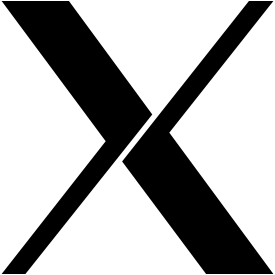
\includegraphics[width=\textwidth]{slides/graphics-software-stack-overview/x11-logo.pdf}
  \end{minipage}
\end{frame}

\begin{frame}{Wayland overview}
  \begin{itemize}
  \item \textbf{Wayland} overview
    \begin{itemize}
    \item Wayland is a \textbf{display protocol} (with a core and extensions), not an implementation
    \item Replaces X11 with a \textbf{less intrusive, more modern and minimal} paradigm
    \item Compositors (server-side) handle \textbf{input, windows, composition and display}
    \end{itemize}
  \end{itemize}
  \begin{minipage}[b]{0.8\textwidth}
  \begin{itemize}
  \item \textbf{Wayland compositor} implementations examples
    \begin{itemize}
    \item Using the \textbf{libwayland-server} base protocol library
    \item \textbf{Weston/libweston}: Reference implementation
    \item \textbf{Sway/wlroots}: Tiling window manager and base library
    \item \textbf{Mutter}: GNOME compositor
    \end{itemize}
  \item \textbf{Display client} libraries
    \begin{itemize}
    \item Using the \textbf{libwayland-client} base protocol library
    \item Integrated in many higher-level graphics-oriented libraries
    \end{itemize}
  \end{itemize}
  \end{minipage}
  \begin{minipage}[b]{0.15\textwidth}
  \includegraphics[width=\textwidth]{slides/graphics-software-stack-overview/wayland-logo.pdf}
  \end{minipage}
\end{frame}

\begin{frame}{High-level graphics libraries and desktop environments overview}
  \begin{minipage}[b]{0.09\textwidth}
  \centering
  \includegraphics[width=\textwidth]{slides/graphics-software-stack-overview/gtk-logo.pdf}\\
  \vspace{3em}
  \includegraphics[width=\textwidth]{slides/graphics-software-stack-overview/qt-logo.pdf}\\
  \vspace{3em}
  \includegraphics[width=\textwidth]{slides/graphics-software-stack-overview/sdl-logo.png}\\
  \vspace{2em}
  \end{minipage}
  \hfill
  \begin{minipage}[b]{0.8\textwidth}
  \begin{itemize}
  \item Applications rarely to never use Wayland or X11 directly
  \item Drawing and managing a user interface is complex
  \item Widely-used high-level graphics libraries (aka toolkits)
    \begin{itemize}
    \item \textbf{GTK} (C): Widget-based UI toolkit, drawing helpers (GDK)
    \item \textbf{Qt} (C++): Widget-based UI toolkit, wide framework
    \item \textbf{EFL} (C): Lightweight UI and application library
    \item \textbf{SDL} (C): Drawing-oriented graphics library (used in games)
    \end{itemize}
  \item A desktop environment groups related libraries and components\\
  \textit{gives a consistent look and feel across the system}
  \item \textbf{Desktop environment} examples
    \begin{itemize}
    \item \textbf{GNOME}: Using GTK, GNOME-Shell desktop
    \item \textbf{KDE}: Using Qt, Plasma desktop
    \item \textbf{Xfce}: Using GTK, lightweight
    \item \textbf{Enlightenment}: Using EFL
    \end{itemize}
  \end{itemize}
  \vfill~
  \end{minipage}
  \begin{minipage}[b]{0.09\textwidth}
  \centering
  \includegraphics[width=\textwidth]{slides/graphics-software-stack-overview/gnome-logo.pdf}\\
  \vspace{1em}
  
\includegraphics[width=\textwidth]{slides/graphics-software-stack-overview/kde-logo.pdf}\\
  \vspace{1em}
  \includegraphics[width=\textwidth]{slides/graphics-software-stack-overview/xfce-logo.pdf}\\
  \vspace{0.5em}
  
\includegraphics[width=\textwidth]{slides/graphics-software-stack-overview/enlightenment-logo.pdf}
  \end{minipage}
\end{frame}
